\chapter{Az OSGi keretrendszerről}
\label{cha:osgi}

Az OSGi Alliance \cite{osgi} által fejlesztett OSGi (\textit{Open Services Gateway initiative}) egy Java nyelvű, dinamikus, szolgáltatás orientált komponens modell és keretrendszer, mellyel kiterjeszthető az alap Java nyelven készült programok funkcionalitása. Használatával elérhető válik egy komponens alapú fejlesztés, ahol alkalmazásokat (illetve komponenseket) távolról elérve telepíthetjük, elindíthatjuk, leállíthatjuk, frissíthetjük, vagy törölhetjük anélkül, hogy a teljes alkalmazást leállítanánk és újra elindítanánk. A standard Java nyelven íródott alkalmazásoknál ez egy fontos hiányosság, hiszen az információs rendszerek sok területén nem engedhetőek meg akár a pillanatnyi leállások sem.

A flexibilitás és újrafelhasználhatóság követelményeknek tehát nagyon jól megfelel az OSGi keretrendszer, ezért is esett rá a választás. Léteznek természetesen más, komponens alapú modelt használó technológiák, például: Microsoft Common Object Model, Enterprise JavaBeans, \mbox{CORBA} Component Model. Ezek közül azonban a legtöbb egy komplex programozási modelen alapul, amely megköveteli konvenciók követését és az OSGi-al szemben nem támogatják a komponensek dinamikus frissítését, így flexibilitás szempontjából ilyen módon elmaradnak.

\begin{figure}[htp]
\centering
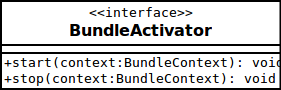
\includegraphics[scale=0.6]{img/class_bundleactivator}
\caption{BundleActivator osztálydiagram}
\label{fig:class_bundleactivator}
\end{figure}

\section{Bundle}
\label{sec:bundle}

Az OSGi technológiát \cite{osgiintro}\cite{hall_challenges_2004}\cite{towardosgi} használó alkalmazások kisebb komponensekre (az OSGI terminológiát használva csomagokra, azaz \textit{bundle}-ökre) vannak bontva. Ezen csomagok elkészíthetőek, lefordíthatóak, telepíthetőek egymástól függetlenül, életciklusukat maga az OSGi keretrendszer felügyeli. A bundle-ök gyakorlatilag nem mások, mint a jól ismert JAR fájlok (Java osztályok, és egyéb erőforrások becsomagolva), azzal a különbséggel, hogy a leíró manifest állományban a szabvány által kiterjesztett módon további fejlécek találhatóak meg. Példát látunk manifest állományra a \ref{lst:manifest}.~kódrészletben. A manifest-ben lévő metaadatok nagy része emberi felhasználás céljából szerepel és nem módosítják az OSGi rendszer működését, kivétel a \texttt{Bundle-Activator} és az \texttt{Import-Package} fejlécek.

A manifest állomány elemei:

\begin{description}
	\item[Bundle-Name] az elkészített bundle emberek számára olvasható neve
	\item[Bundle-SymbolicName] Java package név, ez azonosítja a bundle-t (az egyetlen kötelező elem)
	\item[Bundle-Description] a bundle hosszabb szöveges leírása
	\item[Bundle-ManifestVersion] a bundle által használt OSGi változat verziószáma
	\item[Bundle-Version] a bundle verziószáma
	\item[Bundle-Activator] \texttt{BundleActivator} interfészt implementáló bundle-ben lévő osztály, mely a bundle telepítése után elindul
	\item[Export-Package] más bundle-ök számára elérhetővé tett saját csomagok és verziószámaik listája
	\item[Import-Package] a bundle fordításához és futtatásához szükséges külső csomagok listája
	\item[Private-Package] olyan saját csomagok, amelyeket nem teszünk elérhetővé más bundle-ök számára
\end{description}

A bundle-ök egy OSGi példányon belül, azonos JVM-ben futnak. Ennek vannak előnyei (teljesítmény növekedés, kisebb erőforráshasználat, interprocessz kommunikációt nem szükséges használni), de hátrányai is (hozzáférési problémák), melyeket az OSGi úgy old meg, hogy minden bundle-höz saját classloader-t rendel.

\begin{lstlisting}[label={lst:manifest}, caption=MANIFEST.MF,breaklines=true]
Bundle-Name: Hello World
Bundle-SymbolicName: org.available.helloworld
Bundle-Description: A Hello World bundle
Bundle-ManifestVersion: 2
Bundle-Version: 1.0.0
Bundle-Activator: org.available.helloworld.Activator
Export-Package: org.available.helloworld;version="1.0.0"
Import-Package: org.osgi.framework;version="1.3.0"
Private-Package: org.notavailable.helloworld
\end{lstlisting}

Ha egy komponens kapcsolatba akar lépni az OSGi keretrendszerben lévő más komponenssel, akkor azt a hozzá tartozó egyedi \texttt{BundleContext}-en keresztül teheti meg. A \texttt{BundleContext} megszerzéséhez implementálnia kell a \texttt{BundleActivator} interfészt (\ref{fig:class_bundleactivator}.~ábra), melynek \texttt{.start()} és \texttt{.stop()} metódusainak argumentumaként megkapják a bundle kontextust, illetve előbbi metódusok meghívódnak a komponens indításakor és leállításakor.

% section bundle (end)

\section{Service, Service Registry}
\label{sec:service}

A bundle-ök kiajánlhatnak szolgáltatásokat (\textit{service}), melyekre más bundle-ök feliratkozhatnak. Az OSGi specifikáció szerint a szolgáltatások normál Java objektumok, melyek egy adott interfészt implementálva lettek beregisztrálva az OSGi \textit{Service Registry} moduljába.

A Service Registry segítségével tudnak tehát a bundle-ök kiajánlani szolgáltatásokat, rajtuk keresztül tudják lekérdezni az elérhető szolgáltatásokat. Ha egy bundle-nek szüksége van egy másik bundle által kiajánlott szolgáltatásra, akkor az OSGi keretrendszertől lekéri a \texttt{BundleContext}-en keresztül az adott szolgáltatás referenciáját.

Még robusztusabb használat lehetséges, hogy ha implementáljuk a \texttt{ServiceListener} interfészt (\texttt{.serviceChanged(ServiceEvent e)} metódust), mellyel értesülhetünk a regisztrált illetve eltávolított szolgáltatásokról, így dinamikusan követhetjük a szolgáltatások elérhetőségét, felkészülhetünk például egy hirtelen kieső szolgáltatás kezelésére. Ugyanezt a funkcionalitást elérhetjük másképpen egy \texttt{ServiceTracker} példány használatával is.

A szolgáltatások kezelése ezen módszerek használatával azonban nem skálázódik jól, összetett rendszerekben egyszerűbb technológiák használata jobban kifizetődő. Lássunk tehát néhány példát a szolgáltatások dinamikus kezelésére:

\begin{description}
	\item[Service Binder] A Service Binder komponens létezésének ma már csak történeti okai vannak, mivel a későbbi OSGi R4 specifikációban megjelent újdonságok (Declarative Services, Dependency Manager, iPOJO) teljes mértékben helyettesítik ezt a megoldást. A Service Binder megpróbálja a bonyolult Activator példányok implementációját megkerülni és automatizált módon kezelni a komponens szolgáltatás függőségeit.
	
	A korábbi \texttt{BundleActivator} osztályból való leszármaztatás helyett a \texttt{GenericActivator} osztályból kell leszármaztatni az osztályunkat, és egy XML fájlban deklaratív módon kell meghatározni, hogy milyen szolgáltatás példányokat akarunk létrehozni és azoknak milyen függőségei vannak.
	
\begin{figure}[htp]
\centering
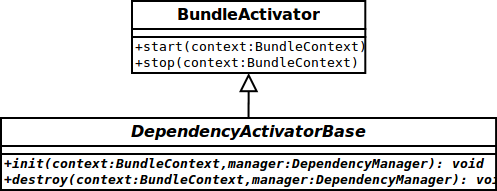
\includegraphics[scale=0.6]{img/class_dependencymanager}
\caption{DependencyManager osztálydiagram}
\label{fig:class_dependencymanager}
\end{figure}

	\item[Declarative Services] A Declarative Services egy komponens model, melynek felépítését befolyásolta a korábbi Service Binder megoldás. A technológia célja, hogy leegyszerűsítse az olyan OSGi komponensek készítését, melyek OSGi szolgáltatásokat használnak.
	
	Fontos jellemzők, hogy használatával nincs szükség explicit módon implementálni a szolgáltatások kiajánlását és felhasználását, ezek deklaratív módon teljes mértékben XML segítségével végezhetőek el. Leszármaztatásra vagy interfész implementációra nincs szükség; a szolgáltatások implementációja a \textit{lazy loading} tervezési mintát követi; a komponensek konfigurációja bármikor megtörténhet Configuration Admin szolgáltatás segítségével.
	
	\item[Dependency Manager] Ebben az esetben a \texttt{DedendencyActivatorBase}-ből kell leszármaztatni az osztályunkat, és implementálni az \texttt{.init()} és \texttt{.destroy()} metódusokat (\ref{fig:class_dependencymanager}.~ábra). A \texttt{DependencyManager} példány segítségével pedig a Decorator mintát használva adhatunk hozzá szolgáltatásokat, és azok függőségeit a komponenshez, valamint konfigurálhatjuk azokat (\ref{lst:dependencymanager_example}.~kódrészlet).

\begin{lstlisting}[label={lst:dependencymanager_example}, caption=Példa a DependencyManager használatára,breaklines=true]
manager.add(createService()
    .setInterface(WebService.class.getName(), null)
    .setImplementation(WebServiceImpl.class)
    .add(createServiceDependency()
        .setService(ConfigurationAdmin.class, null)
        .setRequired(true))
    .add(createServiceDependency()
        .setService(LogService.class, null)
        .setRequired(false));
\end{lstlisting}

    \item[iPOJO] Az iPOJO komponens model központi koncepciója, hogy ne legyen szükség POJO példányoknál bonyolultabb objektumok használatára. Használatát tekintve nagyon hasonló a Declarative Services-hez, azonban az iPOJO kicsit több eszközt kínál a fejlesztőknek. A komponenshez szükséges szolgáltatásokat és azok függőségeit szintén XML fájlban kell deklaratív módon specifikálni, és a rendszer automatikusan kezeli ezeket a függőségeket. Újdonságok a korábbi megoldásokhoz képest például a Java annotációk támogatása, API hozzáférés a belső működéshez, könnyű kiegészíthetőség és beépített távoli konfiguráció JMX segítségével.
 
\end{description}

% section service (end)

\newpage

\section{Életciklus}
\label{sec:lifecycle}

Az OSGi keretrendszer dinamikusságát a \textit{Life-cycle} (életciklus) rendszer szolgáltatja, mely által a bundle-öket futásidőben lehet telepíteni, elindítani, leállítani, frissíteni, eltávolítani más hagyományos alkalmazásokkal ellentétben.

\begin{figure}[htb]
\centering
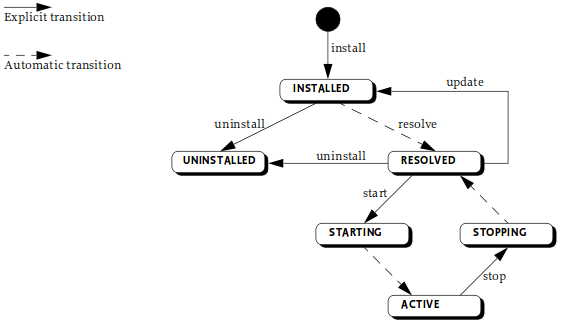
\includegraphics[scale=0.5]{img/bundle_lifecycle}
\caption{Bundle életciklus (forrás: OSGi Service Platform Release 2 \cite{osgi})}
\label{fig:bundle_lifecycle}
\end{figure}

A bundle-ök futtatása előtt megvizsgálja a keretrendszer a csomag futás idejű függőségeit, és ha olyan kielégítetlen függőségeket talál, melyek szükségesek a bundle futtatásához, akkor nem indítja el a komponenst. Egy bundle életciklusának állapotai megfigyelhetőek a \ref{fig:bundle_lifecycle}.~ábrán, valamint az állapotok leírása a \ref{tab:lifecycle_states}.~táblázatban látható.

\begin{table}[htb]
\begin{center}
\begin{tabular}{|L{3cm}|L{10cm}|}
\hline
\textbf{Állapot neve} & \textbf{Leírás} \\
\hline
\hline
INSTALLED   & A bundle sikeres telepítve lett. \\
\hline
RESOLVED    & A bundle-nek minden függősége ki lett elégítve. Kész az elindításra, vagy már le lett állítva. \\
\hline
STARTING    & A bundle el lett indítva, de még nincs aktiválva, .start() metódus még nem tért vissza. \\
\hline
ACTIVE      & A bundle aktiválva lett és aktív. \\
\hline
STOPPING    & A bundle le lett állítva, .stop() metódus még nem tért vissza. \\
\hline
UNINSTALLED & A bundle el lett távolítva, ez az életciklus végállapota. \\
\hline
\end{tabular}
\end{center}
\caption{\label{tab:lifecycle_states} Bundle életciklus állapotai}
\end{table}


% section lifecycle (end)

% chapter osgi (end)